%!TEX root = paper.tex

\section{Auto-context forests for brain tumour segmentation}
\label{sec: cascading}

We investigate cascaded DF architectures, made of layers of DFs partially or fully connected via their output posterior maps. 
%Each layer solves a separate subtask, improves upon the current prediction or both. %DNs form a powerful and flexible meta-framework for high precision vision tasks such as medical image segmentation. 
This architecture naturally interleaves high-level \textit{semantic} reasoning with \textit{intensity}-based low-level 
reasoning. We demonstrate this via two ideas: a) \textit{auto-context}: allowing downstream layers to reason about 
semantics captured in upstream layers, and b) \textit{decision pathway clustering}: latent data-space semantics are 
revealed by clustering \textit{decision pathways} and cluster-specific DFs are trained. 

\subsection{Building and training Auto-Context Forests}

The process of cascading DFs is illustrated in Fig.~\ref{fig: DN concept}. Since DFs rely on generic context-sensitive features %to make statements about likely label assignments, 
that disregard the exact nature of input channels (cf. Section~\ref{sec: features}), we simply proceed by augmenting the set of input channels for subsequent layers with output posterior maps from previous layers. %If $\brmx^{(1)} = \{x,I\}$ is the original data representation, fed to the first DF layer\\

\begin{figure}
\centering
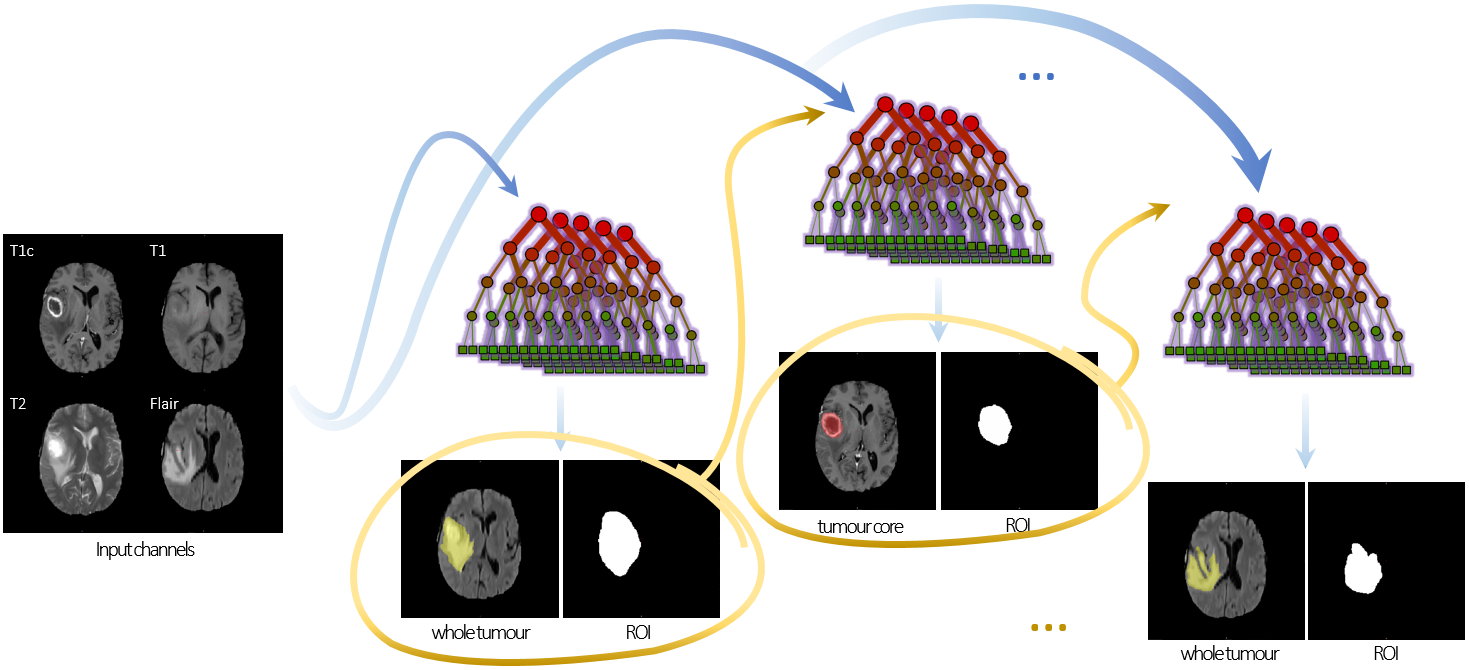
\includegraphics[width=1\columnwidth]{images/DecisionNetwork-BRATS.png}
\label{fig: DN concept}
\caption{Auto-Context Segmentation Forests. In this schematic example, layer $2$ solves a segmentation task distinct from that of layers $1$, $3$ but the interleaving allows to exploit joint dependencies.}
\end{figure}

Layers are trained sequentially, one at a time in a greedy manner (following Sections~\ref{sec: background} and 
\ref{sec: CVE}). 
%The main appeal of the proposed approach is that it is practical, modular, fast and reliable. %We emphasize the following points: a) the ease of adjusting the layer design, of training and tuning individual layers; b) the opportunity to mix DF layers with other forms of processing; and c) the benefit of dividing a challenging hierarchical task into simpler subtasks addressed independently albeit communicating with each other. 
Specifically, for the BRATS challenge, class labels follow a \textit{nested} structure: the whole tumour (WT) 
consists of the edema (ED) and tumour core (TC). The tumour core itself is subdivided into enhancing 
tumour parts (ET), and other parts of the core that are only indirectly relevant to the task: 
the necrotic core (NC) and non-enhancing remaining parts (NE). Usually, 
these labels would be interpreted as mutually exclusive classes (ED, ET, NC, NE and the background BG) 
so as to formulate the task as a multilabel classification problem. 
Instead, our proposed framework directly uses these hierarchical relations. %by interweaving binary DFs. %: end-to-end DN training with joint optimization of layers is feasible, \eg \cite{kontschieder2015deep} but comes at the cost of fixed tree topology and MLE limitations. Comes in the way of fast experimentation, lightweight training and tuning, which we emphasize here.\\
While many variants can reasonably be built, the final architecture that we used for the BRATS challenge consists of layers of binary DFs, alternating between predictions of WT, TC and ET.

%\noindent
%\textbf{Boosting relevant regions.}

\subsection{Exposing Latent Semantics in Decision Forests for guided bagging}
\label{sec: clustering}

%To motivate what follows, consider the example of Fig. \ref{}. The boundary geometry is complex and the dent is likely to be mis-segmented because of misleading contextual cues. Assuming usual loss functions are used, the classifier has little incentive to accurately delineate the boundary: the volume of the boundary region is small, hence few such training samples are seen. %The argument generalizes to subsets of data of low probability w.r.t. the overall data distribution. 
%Datasets %also 
%commonly contain several distinct "clusters" of data, \eg two subtypes of anomalies under identical labels, or subgroups of images with varying acquisition protocols. In that case cluster proportions in the training data are often arbitrary, similarly to the proportions between background and foreground labels. While boosting may partially address the issue, its simplest variants are sensitive to mislabelling in the training data~\cite{long2009adaptive,long2010random} (as commonly occurs in manually annotated datasets) whereas noise-tolerant alternatives remain more intricate and costly. 

Given Auto-Context Forests, a natural idea is to progressively refine the region of interest (ROI) after each layer, starting from an initial over-approximation of the ROI (\eg, the full image). Downstream DFs are trained on 
more refined ROIs that exclude irrelevant background clutter, thereby increasing accuracy. 
%This closely relates to class rebalancing and boosting. ROIs are usually obtained via simple mathematical morphology. 
Such an approach is at risk of excluding false negatives, creating a trade-off between coarser ROIs (high recall) and tighter ROIs (high precision). We investigate a complementary strategy to circumvent this limitation. ROI refinement remains as a computational convenience.

The proposed approach exposes and exploits the latent semantics already captured within a given DF as follows. Each data point is identified with the collection of tree paths that it traverses at test time. A metric $d_{\text{DP}}$ is defined over such collections of tree paths (\textit{decision pathways}), assigning smaller distance between points following similar paths across many trees, and data clusters are identified by $k$-means w.r.t. $d_{\text{DP}}$. % say a word about how the centroid is computed
Then, cluster-specific DFs are trained over the corresponding training data. At test time, data points are assigned to the cluster with closest centroid and the corresponding DF is used for prediction.

Our key insight is that data points that are clustered together will share common underlying semantics, as they jointly satisfy many predicates. A wide range of metrics can be designed and for the sake of simplicity, we define (given a collection $\calT$ of trees):
\begin{equation}
d_{\text{DP}}^{\calT}(\brmx_i, \brmx_j)\triangleq \sum_{t=1}^{\vert\calT\vert} \left(\frac{1}{2}\right)^{\text{depth}_t^{\calT}\!(\brmx_i,\brmx_j)}\, ,
\end{equation}
where $\brmx_i, \brmx_j$ are two points, and $\text{depth}_t^{\calT}(\brmx_i,\brmx_j)$ is the depth of the deepest common node in both paths for the $t$-th tree ($+\infty$ if the paths are identical).
% Figure caption maybe: Given the necessary information, an intuitive solution would be to train a classifier specifically over the boundary region, because cues that are too unreliable over the full image may still be strongly discriminative

% maybe turn it into a single big figure* that shows 1) an illustration of the centroids? 2) the automatically inferred semantics 3) example segmentations with ROI refinement only and with clustering 4) plot the accuracy gain: no ROI refinement vs. 2 settings of ROI refinement only vs the same two settings with clustering, on a suitable example.
